\documentclass[12pt]{report}
\usepackage[utf8]{inputenc}
\usepackage{graphicx}
\usepackage{listings}
\usepackage{threeparttable}
\usepackage{booktabs}
\usepackage{amsmath}
\usepackage{amsfonts}
\usepackage{longtable}
\usepackage{amssymb}
\setcounter{tocdepth}{3}
\setcounter{secnumdepth}{3}
\pagestyle{headings}
\usepackage{algorithm}
\usepackage{algorithmic}
\usepackage{fancyhdr}
\usepackage{qtree}
\usepackage{tikz-qtree}
\usepackage[a4paper, total={6in, 8in}]{geometry}
\pagestyle{fancy}
\usepackage[style=mla,babel=hyphen,backend=biber]{biblatex}
\usepackage {fancybox}
\newtheorem{mydef}{Definition}
\fancyhf{}
\newenvironment{dedication}
  {\clearpage           % we want a new page
   \thispagestyle{empty}% no header and footer
   \vspace*{\stretch{1}}% some space at the top 
   \itshape             % the text is in italics
   \raggedleft          % flush to the right margin
  }
  {\par % end the paragraph
   \vspace{\stretch{3}} % space at bottom is three times that at the top
   \clearpage           % finish off the page
  }

\rhead{\thesection}
\lhead{\leftmark}
\fancyfoot[LE,RO]{\thepage}
\renewcommand{\headrulewidth}{2pt}
\renewcommand{\footrulewidth}{1pt}
\pagenumbering{roman}
\usepackage[nottoc]{tocbibind}
\def\blankpage{%
      \clearpage%
      \thispagestyle{empty}%
      \addtocounter{page}{-1}%
      \null%
      \clearpage}
\begin{document}
\begin{titlepage}

   \begin{center}
   \thisfancypage{%}
\setlength{\fboxsep}{10pt}\doublebox}{}
       \vspace*{1cm}
 	   \Huge
       \textbf{A Game Theoretic Approach for Travel Mode Choice}
		\LARGE
		
       \vspace{0.5cm}
        
            
       \vspace{1.5cm}

       \textit{Fadeli Ismail}
\vfill
\normalsize
Supervisor : KACI Abdellah\\

       \vfill
       
            	\normalsize
       A thesis presented for the degree of\\
       Masters in Transport Engineering
            
       \vspace{0.8cm}
     
       
            \Large
       Department of Transport and Logistics Engineering\\
       National High School of Technology \\
       ENST\\
       Algeria\\
       2020
            
   \end{center}
   

\end{titlepage}
\blankpage
\begin{dedication}\thispagestyle{empty}
Dedicated to 
\end{dedication}
\clearpage
\thispagestyle{empty}
\thispagestyle{plain}
\begin{center}
    \Large
    \textbf{Travel Mode Choice Modeling using Game theory}
        
    \vspace{0.4cm}
    \large
   
        
    \vspace{0.4cm}
    
       
    \vspace{0.9cm}
    \textbf{Abstract}
\end{center}

\clearpage
\section*{Acknowledgment}\thispagestyle{empty}
\clearpage
\tableofcontents \thispagestyle{empty}
\listoffigures
\listoftables
\addcontentsline{toc}{chapter}{Introduction}
\clearpage

\thispagestyle{empty}
\pagenumbering{arabic}
\thispagestyle{empty}
\chapter*{Introduction}
The grow of private vehicle use causes congestion that eventually  increases travel time, this increase pushes governments to motivate people towards public transport. However, more usage of public transport should be followed by an improvement of public transport services.\\

With the intention of making a transport demand analysis, it is essential to understand the traveler's mode choice behavior, where a demand is the accumulation of individuals decisions. The most important element in modeling a transport system is the mode split model, which provides a mathematical framework of the choices a traveler can have of which mode of transport is more suitable.\\

The different objectives in travel mode choice leads to the urge of applying game theory for making decisions based on finding the equilibrium of the passenger choices. However, game theory is rarely used in the transport field with several obstacles appearing in the transport characteristics. But, it is possible to predict the behaviors of travelers? this question has been asked over time, but we still do not have clear answers. Despite the common knowledge that human actions are random and unpredictable, human mobility follows certain patterns.\\

The purpose of this study is to describe how travelers adjust their mode of transport choice behaviors using an evolutionary game model. In evolutionary game theory, a dynamic process is set to describe how players adjust their choices overtime as they learn from the game and also from other players. The present document is organized into three chapters. Chapter 1 describes the basic theories applied in this work, including traditional game theory concepts and evolutionary dynamics. In Chapter 2, key studies from the literature regarding travel choice behavior are briefly examined. The third chapter describes the model used in this study. Limitations of the proposed modeling method and further research directions are discussed at the end. 


\chapter{Game Theory and Evolutionary Dynamics}\setcounter{page}{1}\thispagestyle{empty}
\section{Game Theory}
Game Theory is the study of rational behavior in situations involving interdependence as it may involve:
\begin{itemize}
\item Common interest (coordination);
\item Competing interests (rivalry);
\item Rational behavior: players can do the best they can, in their own eyes;
\item Because of the players' interdependence, a rational decision in a game must be based on a prediction of others' responses;
\end{itemize}
\clearpage

\subsection{The parts of a Game} 
A Game consists of three parts : 
Players, Actions and Payoffs
\subsubsection{Players}
Players are the decision makers and they can be : People, Governments or Companies.
\subsubsection{Actions}
What can the players do ?
Decide when to sell a stock, decide how to vote or enter a bid in an auction...
\subsubsection{Payoffs}
Payoffs can represent the motivation of the players, for example : Do they care about profit ? or Do they care about other players ? 

\subsection{Defining Games} Games can be represented in two methods : Normal forms and Extensive Forms.

\subsection{Extensive Form}
An extensive form game includes timing of moves. 
Players move sequentially, represented as a tree.
\begin{itemize}
\item Chess: white player moves, then black player can see white's move and react...
\end{itemize}
Keeps track of what each player knows when he or she makes a decision :
\begin{itemize}
\item Poker: bet sequentially - what can a given player see when they bet. 
\end{itemize}

\subsection{Normal Form Games}
\paragraph{}A normal form game is a strategic interaction in which each of $n$ players chooses a strategy and the receives a payoff that depends on all agents choices of strategy. In other words, a normal form represents a list of what players get on function of their actions.
Finite, n-person normal form game  ⟨$N, A, u$⟩:
\begin{itemize}
\item Players: $ N = {1, ... , n} $ is a finite set of $n$, indexed by $i$.
\item Actions set for player $i$ $A_i$
\subitem $a = (a_1,...,a_n) \in A = A_1 * ... * A_n $ is an action profile.
\item Utility function or Payoff function for player $i: u_i : A $  $\to$ ${\Bbb{R}}$
\subitem $u = (u_1,..., u_n)$, is a profile of utility functions.
\end{itemize}

\subsection{Best Response and Nash Equilibrium}\label{subsection}
\paragraph{Best Response :}
\begin{equation}\label{eq:1}
 a_i^* \in BR(a_{-i})  iff   \forall a_i \in A_i, u_i(a_i^*,a_{-i}) \geq u_i(a_i, a_{-i})
\end{equation}
 
\paragraph{Nash Equilibrium (Definition):}
$a = <a_1,...,a_n>$ is a "\textbf{pure strategy}" if $\forall i, a_i \in BR(a_{-i})$

\subsection{Dominant strategies}
let $s_i$ and $s_i^`$ be two strategies for player $i$, and let $S_{-i}$ be the set of all possible strategy profiles for other players.
\bigbreak
\title{\textbf{Definitions:} }
\begin{itemize}
\item $s_i$ \textbf{strictly dominates} $s_i^`$ if $\forall s_{-i} \in S_{-i}, u_i(s_i, s_{-i}) \>> u_i(s_i^`, s_{-i})$
\item $s_i$ \textbf{very weakly dominates} $s_i^`$ if $\forall s_{-i} \in S_{-i}, u_i(s_i, s_{-i}) \geq u_i(s_i^`, s_{-i})$
\item A strategy is called \textbf{dominant} if it dominates all others.
\item A strategy profile consisting of dominant strategies for every player must be a Nash Equilibrium.
\end{itemize}

\subsection{Pareto Optimal}
\title{\textbf{Definition:}}
An outcome $o^*$ is \textbf{Pareto-optimal} if there is no other outcome that Pareto-dominates it.

\section{Mixed Strategies and Nash Equilibrium}
\title{\textbf{Definition:}}
A strategy $s_i$ for agent $i$ as any probability distribution over the actions $A_i$.
\begin{itemize}
\item \textbf{pure strategy:} only one action is played with positive probability
\item \textbf{mixed strategy:} more than one action is played with positive probability
\bigbreak
these actions are called the support of the mixed strategy.
\item Let the set of all strategies for $i$ be $S_i$
\item let the set of all strategy profiles be $S = S_1 \times... \times S_n$
\end{itemize}

\subsection{Utility in Mixed Strategies}
In order to find the payoff if all the players follow mixed strategy profile $s \in S$ we can use the \textbf{expected utility} from decision theory: 
\begin{equation} u_i(s) = \sum_{a \in A}u_i(a)P(a|s)\end{equation}
\begin{equation} P(a|s) = \prod_{j \in N}s_j(a_j)\end{equation}

\subsection{Best Response and Nash Equilibrium}The definitions of best response and Nash equilibrium are generalized from actions to strategies. 
\paragraph{Definition (Best Response): }
\begin{equation}
s_i^* \in BR(s_{-i}) \textbf{ if }   \forall s_i \in S_i, u_i(s_i^*,s_{-i}) \geq u_i(s_i, s_{-i})
\end{equation}
\paragraph{Definition (Nash Equilibrium)}
$$s = <s_1,...,s_n>\textbf{ is  a }\textbf{Nash Equilibrium if } \forall i, s_i \in BR(s_{-i})$$
\paragraph{Theorem (Nash, 1950)} Every finite game has a Nash equilibrium.

\subsection{Computing Nash Equilibrium}
\paragraph{Two algorithms for finding NE }
\begin{itemize}
\item LCP(Linear Complimentary) [Lemke-Howson].
\item Support Enumeration Method [Porter et al].
\end{itemize}

\subsection{Complexity Analysis}
\title{\textbf{Theorem:}}
Computing a Nash Equilibrium is a \textbf{PPAD-complete}\footnote{PPAD : Polynomial Parity Argument on Directed Graphs} , this theorem has been proven for:
\begin{itemize}
\item for games $\geq$ 4 players;
\item for games with 3 players;
\item for games with 2 players;
\end{itemize}

\subsection{Summary of mixed strategies}
\begin{itemize}
\item Some games have mixed strategy Nash Equilibria.
\item A player must be indifferent between the actions he or she randomizes over.
\item Randomization happen in business interactions, society, sports...
\end{itemize}

\subsection{Strictly Dominated Strategies}
\paragraph{Definition}a strategy $a_i \in A_i $ is strictly dominated by $a'_i \in A_i$ if
\begin{equation} u_i(a_i, a_{-i}) < u_i(a'_i, a_{-i}) ,  \forall   a_{-i} \in A_{-i} \end{equation}

\subsection{Weakly Dominated Strategies}
\paragraph{Definition}a strategy $a_i \in A_i $ is weakly dominated by $a'_i \in A_i$ if
\begin{equation} u_i(a_i, a_{-i}) \leq u_i(a'_i, a_{-i}) ,  \forall   a_{-i} \in A_{-i} \end{equation}
\begin{center}
and 
\end{center}
\begin{equation} u_i(a_i, a_{-i}) < u_i(a'_i, a_{-i}) ,\exists   a_{-i} \in A_{-i} \end{equation} 

\section{Perfect information games}{The extensive form is an alternative representation that makes the temporal structure explicit.}
\begin{itemize}
\item{Perfect information extensive form games.}
\item{Imperfect information extensive form games.}
\end{itemize}
\title {\textbf{Definition}} A finite perfect information game in extensive form is defined by the tuple ($N, A, H, Z,\chi ,\rho, \sigma, u $)
where:
\begin{itemize}
\item{Players: $N$ is a set of $n$ players.}
\item{Actions: $A$ is set of actions.}
\item{Choice nodes and labels for these nodes: }
\begin{itemize}
\item{Choice nodes: $H$ is a set of non-terminal choice nodes.}
\item{Action function: $\chi : H \to 2^A $ assigns to each choice a set of actions.}
\item{Player function: $\rho : H \to N$ assigns to each non-terminal node $h$ a player $i \in N$ who chooses an action at $h$.}
\end{itemize}
\item{Terminal nodes: $Z$ is a set of terminal nodes, disjoint from $H$.}
\item{Successor function: $\sigma : H \times A \to H \cup Z$ maps a choice node and an action to a new choice node or terminal node such that for all $h_1, h_2 \in H$ and $a_1, a_2 \in A$, if $\sigma(h_1, a_1) = \sigma(h_2, a_2)$ then $h_1  = h_2$  and $a_1 = a_2$} 
\item{Utility function: $u = (u_1,...,u_n)$ where $u_i : Z \to R$
}
\end{itemize} 
\paragraph{}figure \ref{fig:scaled_diss} shows a sharing game represented in the extensive form
\begin{figure}[h]
 
  \centering
  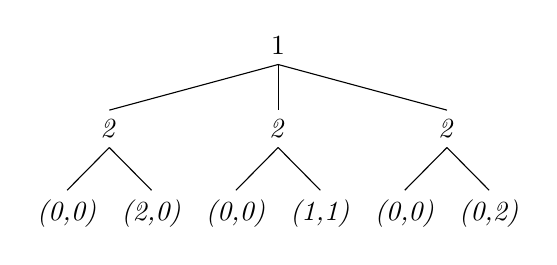
\begin{tikzpicture}[baseline] % baseline makes the example number stay at the top of the tree
   \Tree[.1 [.\textit{2 } [.\textit{(0,0) } ] [.\textit{(2,0) } ]][.\textit{2 } [.\textit{(0,0) } ] [.\textit{(1,1) } ]][.\textit{2 } [.\textit{(0,0) } ] [.\textit{(0,2) } ]]]
     \end{tikzpicture}%
  \caption{Sharing Game\label{fig:scaled_diss}}
\end{figure}
\subsection{Pure Strategies}
\paragraph{} A pure strategy for a player in a perfect-information game is a complete specification of which action to take at each node belonging to that player.
\paragraph{Definition} Let $G = (N, A, H, Z,\chi ,\rho, \sigma, u ) $ be a perfect-information extensive-form game. Then the pure strategies of player $i$ consist of the cross product\\
\begin{center}
$ \prod_{h \in H, \rho(h)=i}\chi(h)$
\end{center}
\paragraph{}
Given our new definition of pure strategy, we can reuse our old definitions of mixed strategies and Nash equilibrium in \ref{eq:1}.

\subsection{Sub-game Perfection}
\begin{mydef}[Sub-game Perfection]\label{def:def555}
The set of sub-games of $G$ is defined by the sub-games of $G$ rooted at each of the nodes in $G$.
\end{mydef}
\paragraph{}Let $s$ be a  sub-game perfect equilibrium of $G$ if for any sub-game $G'$ of $G$, the restriction of $s$ to G' is a Nash Equilibrium of $G'$. Since $G$ is its own sub-game , every sub-game perfect is a Nash Equilibrium.

\subsection{Backward Induction}

\begin{algorithm}{h}
\caption{Backward Induction\label{fig:scaled_back}}
\begin{algorithmic}
\RETURN $u(h)$
\IF{$h \in Z$}
\RETURN{$u(h)$}
\ENDIF
\STATE $best-util \leftarrow -50$
\FORALL{$a \in \rho(h)$} 
\STATE $util-at-child \leftarrow BACKWARDINDUCTION(\sigma(h,a))$ 
\IF{$util-at-child_p(h) >best-util_p(h)$}
\STATE $best-util \leftarrow util-at-child$
\ENDIF
\ENDFOR
\RETURN $best-util$
\end{algorithmic}
\end{algorithm}
\paragraph{}Backward Induction has been used in solving games since John von Neumann and Oskar Morgenstern published their book, Theory of Games and Economic Behaviors in 1944.
\paragraph{}The idea behind Backward Induction is to identify the equilibrium in the buttom trees, and adopt these as one moves up the tree as the next algorithm shows.


\paragraph{} Denote $util_at_child$ is a utility vector for each player.
\section{Evolutionary Game Theory}

\paragraph{}Evolution and Game Theory was introduced by John Maynard Smith in Evolution and The Theory of Games. The Theory was formulated to understand the behavior of animals in game theoretic situations. But it can be applied to modeling human behavior.

\paragraph{}After the emergence of traditional game theory, biologists realized the potential of game theory to formally study adaptation and convolution of biological populations, especially in contexts where the fitness of a phenotype depends on the composition of the population (Hamilton, 1967). The main assumption of evolutionary game theory was that strategies with greater payoffs at a particular time would tend to spread more and thus have better chances of being present in the future.
\paragraph{}The most important concept of evolutionary thinking that was introduced by Manynard Smith and Price (1973) is the notion of \textbf{Evolutionary Stable Strategy}(ESS), for 2-player symmetric games played by individuals belonging to the same population. Furthermore, a strategy $s$ is an ESS if and only if, when adopted by all members of a population, meaning that any other strategy $i$ that could enter the population in a low percentage would obtain a strictly  lower expected payoff in the population than the $s$ strategy.
\paragraph{}The basic ideas behind Evolutionary game theory is that strategies with greater payoffs tend to spread more, and that fitness is frequency dependent soon transcended the borders of biology and started to spread through many other disciplines. In economic context, it was understood that natural selection would derive from competition among entities for small resources or market shares. In social contexts, evolution was often understood as cultural evolution, and it referred to dynamic changes in behavior or ideas over time (\cite{Nelson and Winter, 1982})(\cite{Boyd and Richerson, 1985}).
\paragraph{}In order to extend this understanding further, let's consider this example:
Suppose that a small group of mutants choosing a strategy different from $\delta$* to enter the population.
\begin{itemize}
\item Denote the fraction of mutants in the population by $\varepsilon$ and assume that the mutant adopts the strategy $\delta$.
\item The expected payoff of a mutant is : 
	$(1-\varepsilon)u(\delta,\delta*)+\varepsilon u(\delta*,\delta)$
\item The expected payoff of a mutant that adopts the strategy is :	\\
	$(1-\varepsilon)u(\delta*,\delta*)+\varepsilon u(\delta*,\delta)$
	\item For any mutation to be driven out of the population we need the expected payoff of any mutant to be less than the expected payoff of normal organism :\\
	\begin{equation}(1-\varepsilon)u(\delta*,\delta*)+\varepsilon u(\delta*,\delta) > (1-\varepsilon)u(\delta,\delta*)+\varepsilon u(\delta*,\delta)  \end{equation}
\end{itemize}
\subsection{Static Notions of Evolutionary Stability}
\paragraph{}Maynard Smith offered a stability concept for populations of animals sharing a common behavioral trait, that of player a mixed strategy in  the game. Maynard defines such a population as stable if it is resistant to invasion by a small group of mutants carrying a different strategy(Sandholm, 2017).
\paragraph{}Suppose that a large population is randomly matched to play the symmetric normal form game $A$. We call a mixed strategy $x \in X$ an \textbf{evolutionarily stable strategy} (ESS) if 
\begin{equation}\label{eq:5}
x' A((1 - \epsilon)x + \epsilon y) > y' A((1 - \epsilon)x + \epsilon y) 
\end{equation}
\begin{center}
$\forall \epsilon \leq \epsilon(y)$ and $y \neq x.$
\end{center}
\paragraph{}In order to explain condition \ref{eq:5}, let's consider a population programmed to play mixed strategy $x$ is invaded by a small group of mutants programmed to play the alternative mixed strategy $y$. Equation \ref{eq:5} requires that regardless of the choice of $y$, an incumbent's expected payoff from a random match in the post entry population exceeds that of a mutant so long as the size of the invading group is sufficiently small.
\paragraph{}The definition of ESS above can also be expressed as a combination of two conditions: 
\begin{equation}\label{eq:6}
x' A x \geq y' A x  \: \forall  \: y \in X
\end{equation}
\begin{center}
For all $y \neq x.$
\end{center}
\begin{equation}\label{eq:7}
[x' A x = y' A x] \implies [x' A y > y' A y]
\end{equation}
\paragraph{}Condition \ref{eq:6} requires that the incumbent strategy $x$ be a best response to itself. Condition \ref{eq:7} requires that if a mutant strategy $y$ is an alternative best response against the incumbent strategy $x$ then the incumbent ears a higher payoff against the mutant than the mutant earns against itself.
\paragraph{}Maynard Smith's notion of ESS attempts to capture the dynamic process of natural selection using a static definition.

\section{Population Games}
\paragraph{}Population games provide a simple and general framework for studying strategic interactions in large populations whose members play pure strategies. The simplest population games are generated by random matching in normal form games, but the population game framework allows for interactions of a more intricate nature.
\paragraph{}We focus here on games played by a single population. All agents in this game play equivalent roles. We suppose that there is a unit mass of agents, each of whom chooses a pure strategy from the set
 $S = {1, ... , n}$. The aggregate behavior of these agents is described by a population state $x \in X$, with $x_j$ representing the proportion of agents choosing pure strategy $j$. We identify a population game with a continuous vector valued payoff function $ F:X \rightarrow R^n$. The scalar $F(x)$ represents the payoff to strategy $i$ when the population state is $x$.
\paragraph{}Population state $x^*$ is a Nash Equilibrium of $F$ if no agent can improve his payoff by unilaterally switching strategies.

\chapter{Literature Survey and Methodology} 



\paragraph{}The current approach to mode choice behavior
in the perspective of expected utility theory or random utility theory. However, travelers evaluate the alternative modes by individual experience and attitude which are not considered in the expected utility theory or random utility theory models. Therefore, many alternative theories have been proposed, for example, prospect theory, cumulative prospect theory and regret theory. Among them, cumulative prospect theory draws the most attention because it describes the bounded rational behaviors under various conditions.
\section{Travel Demand Management}
One of the most important socio-economic problems in recent decades has been the optimization of an urban transport system. Furthermore, This type of problem mainly occurs in developing countries, and the reason behind it is the increasing rate of car ownership.\footnote{Khovako, 2014,.}. Which urges cities to realize transport strategies combating this effect and also to decrease the negative impacts of transportation on the environment \footnote{World Bank, 2011}.

\section{Choice Decision Elements}
\paragraph {}The framework for the choice process is that the individual determines the available alternatives(modes), next, evaluates the attributes of each alternative, and then, uses a decision rule to select an alternative from among the available alternatives (Ben-Akiva and Lerman, 1985, Chapter 3).\\
Further in this section, we see that the elements of a choice process are : the decision maker, the alternatives, the attributes of alternatives and the decision rule.


\chapter{Model and Analysis}

\paragraph{}The contribution of this study on mode choice in transportation is in the following ways: 
(1) the research on modeling choices in travel mode selection using game theory concepts, (2) 
\clearpage

\section{Evolutionary Game Theory and Travel Mode Choice}
\paragraph{}Evolutionary game theory is used in this paper as a vehicle for discussing travel mode choice based on the following apparent similarities: 
\paragraph{}A group can be a substitute for an individual as a participant in evolutionary game theory, and the proportions of the individuals choosing different pure strategies in the group can substitute for mixed strategy. The results of travel mode choice are group behavior within the travel mode subsystems, and the only proportions of individuals choosing each travel mode are meaningful for management and study.
\paragraph{}Group Nash equilibrium means that the frequency of the adopted strategies makes the strategy payoffs exactly equal with no one desiring a change in strategy, then the percentage of individuals choosing each different strategy remains stable and reaches equilibrium. In the stable travel context, a travel mode choice will tend to be stable, the Nash equilibrium of the evolutionary game will be changed by the means of traffic control, the construction, and the structure of the transportation system.
\paragraph{}The nature of group strategies acts is that only a bounded rationality human gets closer to Nash equilibrium by summarizing their experience and adjusting their strategies rather than by using a perfectly rational method and Nash equilibrium analysis as reasoning. The players can obtain information such as travel time, travel cost, and traffic information, and they can observe the historical results and the strategies adopted by others. The inhabitants observe and experience the service provided by trip modes during their frequent travels and finally determine their strategies. Although they are bounded by rationality, constantly repeated travel leads the structure of travel mode choice by modes to reach excellent stability.
\subsection{Evolutionary Game Model}
\paragraph{} The extensive form of the sequential, the game displayed in Figure 1, describes the process of travel mode choice. Two conditions have been implemented in this model.
\begin{itemize}
\item Travelers can be divided into two main categories: car owners and noncar owners. As mentioned before, travel is a two stage process, first, every player chooses whether they own a car or not; then, the car owners will select from one of four modes: car, taxi, bus, or rail, and the noncar owners will only select from taxi, bus, or rail.
\item The payoff function that inhabitants must contribute is independent of the proportion of inhabitants traveling in a particular mode.

\end{itemize}
\paragraph{} As mentioned in Chapter 1, the extensive form is defined by three  main objects.
\begin{itemize}
\item the set of players $N = {1,...,n}$, all travelers are players.
\item The strategy sets of the players are $S_1 = {Car owneer, Noncar owner}$ and ${S_2 = {Travel by car, Travel by taxi, Travel by bus, Travel by rail}}$.
\item The payoff functions of the players are $f_{car} = v_1$, $f_{taxi} = v_2$, $f_{bus} = v_3$, and $f_{rail} = v_4$
\end{itemize}
\paragraph{}Players use mixed strategy, because it is impossible for them to travel using the same pure strategy mode multiple times with certainty.
\paragraph{}As explained in Chapter 1, the mixed strategy happens when an individual plays one of the pure strategies of a game with a continuous probability $p$ between 0 and 1. As a result, the payoff the of the individual using mixed strategy depends on the probabilities of the mixed strategy.
\paragraph{}Figure 3.1 shows the game model of travel mode choice, we note that in stage 1 of the game $p_c$ and $p_n$ are the probabilities of car owners and non car owners respectively. In stage 2, $p^c_{c}$, $p^{c}_{t}$, $p^c_{b}$, and $p^c_{r}$ are the respective probabilities of car owner traveling by car, taxi, bus or rail. The probabilities of the noncar owner traveling by taxi, bus or rail are $p^n_{t}$, $p^n_{b}$, and $p^n_{r}$.


\chapter*{Conclusion}
The goal of this project was to build a travel mode choice model capable of embedding game theory, the simulation model can be used in further research as a starting point. The model assumes that the travelers use mixed strategy when making choices, hence, the probability of a mode being chosen is dynamic. \\

\paragraph{}
The simulations used in this work modeling a set of travelers in making choices of two modes : car or public transport. This model is based on a split mode framework often used to describe the choice behavior of travelers.
\paragraph{}
Game theory has proven its usefulness in modeling the relationship between travel mode choices and their payoffs through Nash Equilibrium. An increase in a mode's payoff can increase its proportion. The evolution part of this study is the change in Nash Equilibrium of travel mode choice.
\paragraph{}
Although people often use multimodal transport, combining two or more travel modes in the same trip, which this model lacks. This mechanism is often used to avoid traffic or lack of coverage in some areas.
\paragraph{}Finally, borrowing concepts from machine learning and artificial intelligence studies, we can use neural networks and genetic algorithms to represent the decision making process and consequent behaviors of travelers. Instead of fixed rules governing the way an individual makes decisions. It would also be interesting to add more components besides the ones that this travel mode choice model have, which can be done by further research. Studying the dynamics of travel mode choice behavior could also extract new patterns that can be out of the scope of this model.

\begin{thebibliography}{2}
\bibitem{Boyd and Richerson, 1985}
Boyd, R. and Richerson, P. J. (1985). Culture and the Evolutionary Process. University of Chicago Press.
\bibitem{Maynard} 
Maynard Smith, J. (1982). Evolution and the Theory of Games. Cambridge University Press, Cambridge.
\bibitem{Bravo et al, 2009}
Bravo et al, (2009) An integrated behavioral model of the land-use and transport systems with network congestion and location externalities. Transportation Research Part B. pp. 584-596.
\bibitem{smith} 
Maynard Smith, J. and Price, G. R. (1973). The logic of animal conflict. Nature, 246:15–18. 
\bibitem{Quijano et al, 2017}
Quijano, N., Ocampo-Martinez, C., Barreiro-Gomez, J., Obando, G., Pantoja, A., and Mojica-Nava, E. (2017). The role of population games and evolutionary dynamics in distributed control systems: The advantages of evolutionary game theory. IEEE Control Systems Magazine, 37(1):70–97.
\bibitem{Litman,2011}
Litman, T. (2011). Why and how to reduce the amount of land paved for roads
and parking facilities. Environmental Practice. 13(1), pp. 38-46.
\bibitem{Marden and Shamma, 2015} 
Marden, J. R. and Shamma, J. S. (2015). Game theory and distributed control. In Young, H.P. and Zamir, S., editors, Handbook of Game Theory with Economic Applications, volume 4, chapter 16, pages 861–899. Elsevier, Amsterdam.
\bibitem{Nelson and Winter, 1982}
Nelson, R. R. and Winter, S. G. (1982). An Evolutionary Theory of Economic Change. Harvard University Press.

\bibitem{Richard, David, 1982}
Richard, B. David, M. and Richard, W(1982). A Selective Review of Travel-Mode Choice Models, pp. 370-375.
\bibitem{Jackson, Leyton-Brown and Shoham; 2013}
Jackson, Leyton-Brown and Shoham, 2013 . Game Theory, https://www.coursera.org/learn/game-theory-1/, accessed on May 2020. 

\bibitem{Von Neumann, and Morgenstern, 1944}
Von Neumann, J. Morgenstern ,O, (1944). Theory of games and economic behavior. Princeton University Press.
\end{thebibliography}

\end{document}